\documentclass[cs4size,a4paper]{ctexart}
%==================== 中文字体 ============
% \newcommand\timesnewroman{font/TimesNewRoman/TimesNewRoman-Regular.ttf}
% \newcommand\timesnewromanb{font/TimesNewRoman/TimesNewRoman-Bold.ttf}
% \newcommand\sourcehanserif{font/SourceHanSerif/SourceHanSerifSC-Regular.otf}
% \newcommand\sourcehanserifb{font/SourceHanSerif/SourceHanSerifSC-Bold.otf}
% \newcommand\firacode{font/FiraCode/FiraCode-Regular.otf}
% \newcommand\firacodeb{font/FiraCode/FiraCode-Bold.otf}

\setmainfont[Mapping=tex-text]{Times New Roman}
\setsansfont[Mapping=tex-text]{思源黑体 Regular}
\setmonofont{Fira Code}

%% 中文字体
\setCJKmainfont[BoldFont={思源宋体 Bold}, ItalicFont={AR PL UKai CN}]{Source Han Serif SC}
\setCJKsansfont[BoldFont={思源黑体 Bold}]{思源黑体 Regular}
\setCJKmonofont{AR PL UKai CN}       % macos word

\xeCJKsetup{CJKmath=true}
\setCJKmathfont{AR PL UKai CN}  % 数学环境中使用楷体
%==================== 数学符号公式 ============
\usepackage{amsmath}                 % AMS LaTeX宏包
\usepackage[style=1]{mdframed}
\usepackage{amsthm}
\usepackage{amsfonts}
\usepackage{mathrsfs}                % 英文花体字 体
\usepackage{bm}                      % 数学公式中的黑斜体
\usepackage{bbding,manfnt}           % 一些图标,如 \dbend
\usepackage{lettrine}                % 首字下沉,命令\lettrine
\def\attention{\lettrine[lines=2,lraise=0,nindent=0em]{\large\textdbend\hspace{1mm}}{}}
\usepackage{longtable}
\usepackage[toc,page]{appendix}
\usepackage{geometry}                % 页边距调整
\geometry{top=3.0cm,bottom=2.7cm,left=2.5cm,right=2.5cm}
%====================公式按章编号==========================
\numberwithin{equation}{section}
\numberwithin{table}{section}
\numberwithin{figure}{section}
%================= 基本格式预置 ===========================
\usepackage{fancyhdr}
\pagestyle{fancy}
\fancyhf{}
\fancyhead[C]{\zihao{5}  \kaishu 中期检查报告 - 李源勋}
\fancyfoot[C]{~\zihao{5} \thepage~}
\renewcommand{\headrulewidth}{0.65pt}
\CTEXsetup[format={\centering\bfseries\zihao{-2}},name={, }]{section}
\CTEXsetup[nameformat={\bfseries\zihao{3}}]{subsection}
\CTEXsetup[nameformat={\bfseries\zihao{4}}]{subsubsection}
%================== 图形支持宏包 =========================
\usepackage{subfigure}
\usepackage{graphicx}                % 嵌入png图像
\usepackage{color,xcolor}            % 支持彩色文本、底色、文本框等
\usepackage{hyperref}                % 交叉引用
\usepackage{caption}
\usepackage{url}
\usepackage{multirow}
\captionsetup{figurewithin=section}
%==================== 源码和流程图 =====================
\usepackage{listings}                % 粘贴源代码
\usepackage{xcolor}
\usepackage{color}
\definecolor{dkgreen}{rgb}{0,0.6,0}
\definecolor{gray}{rgb}{0.5,0.5,0.5}
\definecolor{mauve}{rgb}{0.58,0,0.82}

%--------------------
\hypersetup{hidelinks}
\usepackage{booktabs}
\usepackage{shorttoc}
\usepackage{tabu,tikz}
\usepackage{float}

\usepackage{multirow}

\tabcolsep=1ex
\tabulinesep=\tabcolsep
\newlength\tikzboxwidth
\newlength\tikzboxheight
\newcommand\tikzbox[1]{%
        \settowidth\tikzboxwidth{#1}%
        \settoheight\tikzboxheight{#1}%
        \begin{tikzpicture}
        \path[use as bounding box]
                (-0.5\tikzboxwidth,-0.5\tikzboxheight)rectangle
                (0.5\tikzboxwidth,0.5\tikzboxheight);
        \node[inner sep=\tabcolsep+0.5\arrayrulewidth,line width=0.5mm,draw=black]
                at(0,0){#1};
        \end{tikzpicture}%
        }

\makeatletter
\def\hlinew#1{%
  \noalign{\ifnum0=`}\fi\hrule \@height #1 \futurelet
   \reserved@a\@xhline}

\newcommand{\tabincell}[2]{\begin{tabular}{@{}#1@{}}#2\end{tabular}}%

\usepackage{subfigure}
\usepackage{ifthen}


\usepackage{graphicx}
\newcommand{\HRule}{\rule{\linewidth}{0.5mm}}

\newtheorem{Theorem}{定理}
\newtheorem{Lemma}{引理}
%%使得公式随章节自动编号
\makeatletter
\@addtoreset{equation}{section}
\makeatother
\renewcommand{\theequation}{\arabic{section}.\arabic{equation}}

%-------------------------
\usepackage{pythonhighlight}
\usepackage{tikz}
\usepackage{tikz-3dplot}
\usetikzlibrary{shapes,arrows,positioning}
%===================   正文开始    ===================
\begin{document}
\bibliographystyle{gbt7714-2005}     %论文引用格式
%===================  定理类环境定义 ===================
\newtheorem{example}{例}              % 整体编号
\newtheorem{algorithm}{算法}
\newtheorem{theorem}{定理}            % 按 section 编号
\newtheorem{definition}{定义}
\newtheorem{axiom}{公理}
\newtheorem{property}{性质}
\newtheorem{proposition}{命题}
\newtheorem{lemma}{引理}
\newtheorem{corollary}{推论}
\newtheorem{remark}{注解}
\newtheorem{condition}{条件}
\newtheorem{conclusion}{结论}
\newtheorem{assumption}{假设}
%==================重定义 ===================
\renewcommand{\contentsname}{目录}
\renewcommand{\abstractname}{摘要}
\renewcommand{\refname}{参考文献}
\renewcommand{\indexname}{索引}
\renewcommand{\figurename}{图}
\renewcommand{\tablename}{表}
\renewcommand{\appendixname}{附录}
\renewcommand{\proofname}{证明}
\renewcommand{\algorithm}{算法}
%============== 封皮和前言 =================
\begin{titlepage}

\begin{center}


% Upper part of the page
\includegraphics[width=0.65\textwidth]{figure/logo}\\[2cm]    

\textsc{\LARGE Xi'an Jiaotong University}\\[1.5cm]

{\Large \textbf{中期检查报告}}\\[0.5cm]


% Title
\HRule \\[0.7cm]
{ \huge \bfseries 面向多CPU集群的深度行人重识别研究}\\[0.4cm]

\HRule \\[1.5cm]

\Large \underline{~电信~}学院\underline{~计算机~}系\underline{~44~}班 \\[1cm]

\begin{center}
\begin{Large}
\begin{tabular}{cc}
学生姓名:& 李源勋\\ \cline{2-2}\\
学\qquad 号:&~~~~~2140505083~~~~~\\ \cline{2-2}\\
指导老师:& 何~~晖\\ \cline{2-2}\\
\end{tabular}
\end{Large}
\end{center}

\vfill

% Bottom of the page
{\large \today}

\end{center}

\end{titlepage}

\pagestyle{plain}
\pagenumbering{Roman}

%============== 论文正文   =================
\pagestyle{fancy}
\pagenumbering{arabic}
\section{项目背景及内容}
随着视频监控技术的发展,无人值守的视频监控设备被越来越普遍地部署在国民社会的各个方面,在
公安、交通、智能楼宇、金融、司法、教文卫等领域都有着不可替代的作用。具体的应用场景包括平
安城市、卡口系统、工地监控、自助银行、监狱劳教和学前教育等。

在视频监控领域一个很重要且极具挑战性的问题是行人的重识别。行人重识别,指的是在多个视野不
重叠的监控视频中,重新识别那些之前出现过的行人,即把当前行人与之前已标记的人物相对应。该
工作的实现可以为人物搜索、特定人物跟踪等应用提供强有力的支持,进而应用在平安城市、工地监
控、学前教育等场景。

行人重识别技术在实际应用中受诸多因素的影响,包括摄像头的部署位置、成像质量以及摄像头数量
等等。面对一个从未部署过摄像头的监控场景,一个优秀的摄像头位置部署方案可以实现监控范围无
死角、行人重识别准确率高以及跨摄像头持续跟踪的连续性强。摄像头的成像质量受其自身的性能参
数影响,同时也受部署位置的光线条件影响。在理想情况下,摄像头的数量越多,得到的行人信息就
越多,更有利于行人重识别算法的实施。但是在预算有限的情况下,摄像头的数量不可能无限增加。
因此,如何选择摄像头的数量及其部署位置,使得行人重识别算法的性能最大化,便成为一个极具现
实意义的研究问题。

要实现行人的重识别需要借助计算机视觉领域的技术。目前的计算机视觉算法的前沿关注点主要集中
在深度学习技术。由于深度学习的海量计算需求和GPU强大的并行计算能力,大部分深度学习模型都
是借助GPU来调整模型参数。然而使用GPU进行运算也存在许多问题,例如GPU设备通常比较昂贵,
且少见于嵌入式设备中。同时GPU的显存普遍不高,限制了模型的规模以及每一批次数据的规模。与
此同时,多CPU集群具有硬件成本低、搭建方式灵活以及部署广泛等优点,然而对于深度学习算法在
多CPU集群上的研究与应用少之又少。因此,有必要对深度学习算法在多CPU集群上的性能表现进行
深入的调查、分析和研究。

基于上述研究背景及动机,本项目的主要研究内容和贡献如下:

\begin{enumerate}
\item 深入理解论文\cite{sun2017beyond}的目的、想法和实现方式,并使用PyTorch深度学习框架
复现,达到与原论文接近的实验结果。
\item 研究在预算有限的情况下,摄像头的数量与部署位置对行人重识别算法的影响,并采用强化学习
算法进行摄像头部署位置的选择。
\item 调查、分析和研究深度行人重识别算法在多CPU集群上的性能表现,提出针对多CPU集群环境
的深度神经网络模型的改进策略。
\end{enumerate}

本项目当前的进展:

\begin{enumerate}
\item 搭建了PyTorch分布式环境,完成了论文复现工作,在Market1501\cite{zheng2015scalable}
数据库上进行实验。
\item 实现了 Q-Learning 强化学习算法,选择最优的摄像头部署方案。
\item 将深度行人重识别模型的训练算法改造成适用于多CPU集群的形式。
\end{enumerate}

























      %
\section{前期准备}
项目的前期准备主要包括天河二号实验平台的搭建和当前行人重识别领域state-of-the-art的复现。
\subsection{天河二号实验平台的搭建}

\subsubsection{天河二号实验平台参数}

天河二号拥有约17920个计算节点,每个通用节点配备两颗Xeon E5系列12核心的中央处理器、三个Xeon
Phi 57核心的协处理器(运算加速卡),总内存容量约1.4PB,全局存储总容量约12.4PB
\cite{tianhe2018config}。2017年9月,天河二号启动升级工程,二期系统天河二号A采用国产加速器
Matrix 2000,替换原有的Xeon Phi 57加速器,升级后系统峰值运算速度将达到94.97Pflops
\cite{tianhe2017summary}。天河二号各分区的详细配置如表\ref{tab:tianheconfig}。

本项目使用了天河二号的GPU分区,与其它分区最大的不同在于GPU分区每个节点都配备了2块NVIDIA
Tesla K80显示卡,显示内存VRAM为24GB,单精度浮点数运算速度为 8.74 TFLOPS,双精度浮点数的运
算速度为 2.91 TFLOPS。每个节点同时具备高性能的CPU和GPU运算能力,方便进行深度神经网络模型训练
的对比测试。与此同时,各节点之间通过千兆网络进行连接,可用于搭建多节点分布式计算网络。

天河二号的节点分为登陆节点和计算节点。登陆节点主要用于代码编译、数据解压、环境配置等工作。计算
节点配备了高性能的CPU和GPU,主要用于大数据计算,以及大规模的编译任务。登陆节点和计算节点的操
作系统均为 CentOS 7,系统使用slurm作业管理系统管理作业队列,使用module管理各种可选的软件包、
运行库。

\subsubsection{软件编译安装}

由于天河二号的登陆节点和计算节点均不能连接互联网,同时普通用户也没有直接安装软件的权限,
所以需要将必要的软件先在本地完成安装,再通过FTP协议将二进制文件打包传输到天河二号上。

由于需要复现的模型在结构上比较独特,训练方式也千奇百怪。对于 Caffe 和 TensorFlow 这样的
预编译框架,不灵活这一缺陷就变得十分明显了。

而这方面正是 PyTorch 的强项,它是一个非常 Pythonic 的深度学习框架,一切的操作(包括模型
的定义、训练、测试)都十分地符合 Python 的简单的哲学,可以非常轻松快速地构建出一个十分怪
异的模型,非常适合科研人员。

\subsubsection{安装Anaconda}

安装Anaconda十分简单,只需要从官网上下载相应平台的安装包,直接执行安装即可。

\subsubsection{安装CUDA和cuDNN}

CUDA采用最新的9.0版本,直接从NVIDIA官网下载安装即可。cuDNN需要注册开发者账户并填写问卷
即可下载安装。

\subsubsection{安装PyTorch}

在Anaconda里创建独立的Python3 env,然后执行
conda install pytorch torchvision cuda90 -c pytorch 即可。

\begin{table}[]
\centering
\caption{天河二号各分区配置表:天河二号的节点分别属于三个分区:CPU分区、GPU分区和胖节点分区。
其中CPU分区内的节点数量最多,是天河二号的计算主力,每个节点配备了2块12核的Intel Xeon E5-2692
处理器以及64GB内存,既能通过分布式联合满足大型计算的需求,又能保持在小型计算中节能的优势。GPU
分区的特点是每个节点配备了2块NVIDIA Tesla K80显示卡,每张显示卡的VRAM为24GB,同时节点的通
用RAM为256GB,可以很好地满足大量图像处理、图形渲染的需求。胖节点分区的节点配备了足够大的内存,
同时对于CPU也进行了升级,满足特定计算场景下的特殊需求。}

\label{tab:tianheconfig}
\begin{tabular}{|c|c|c|c|c|}
\hline
\multicolumn{2}{|c|}{节点/分区}  & CPU                          & 内存    & GPU                  \\ \hline
\multicolumn{2}{|c|}{CPU分区}  & 2 $\times$ 12 Intel Xeon E5-2692 v2 & 64GB  & -                    \\ \hline
\multicolumn{2}{|c|}{GPU分区}  & 2 $\times$ 10 Intel Xeon E5-2660 v3 & 256GB & 2 $\times$ NVIDIA Tesla K80 \\ \hline
\multirow{3}{*}{胖节点} & 128GB & 2 $\times$ 12 Intel Xeon E5-2692 v2 & 128GB & -                    \\ \cline{2-5}
                     & 3TB   & 4 $\times$ 14 Intel Xeon E7-4850 v3 & 3TB   & -                    \\ \cline{2-5}
                     & 6TB   & 8 $\times$ 16 Intel Xeon E7-8867 v3 & 6TB   & -                    \\ \hline
\end{tabular}
\end{table}

\subsection{数据采集}

要研究摄像头的数量与部署位置对行人重识别算法的影响,数据集需要满足以下要求:一、数据集中摄像头的个数需要超过10个,以便控制增减摄像头的进行分析对比,分析摄像头的拍摄位置对于监控效果的影响;二、存在视野重叠或拍摄位置接近的摄像头,以便分析同一位置、不同拍摄角度的拍摄方案对于监控效果的影响。三、行人需要出现在多个(而不仅仅是两个)摄像头画面内,且摄像头的分布呈路线状(可以存在分支),这样更符合行人跟踪的定义,更好地评估摄像头部署位置的监控效果。

表\ref{tab:reiddataset}是对当前行人重识别领域常见数据库的统计。从表中可以看到在当前主流数据中,VIPeR\cite{gray2007evaluating}、CUHK01\cite{li2012human}、Market1501\cite{zheng2015scalable}和DukeMTMC-reID\cite{ristani2016MTMC}数据集中摄像头数量较少,不利于分析增减摄像头以评估摄像头数量对监控效果的影响。包括CUHK03\cite{li2014deepreid}在内的所有数据集都缺乏单个行人持续追踪的场景,不利于实现监控效果的评估。

因此,有必要针对上述需求重新采集一个数据库,满足研究和实验的需求。经过路线规划、场地布置、演员召集等工作,目前完成了数据库的预拍摄工作。数据集的正式拍摄计划与2018年5月18日和19日进行,计划召集500余名演员参与。第一次预拍摄过程的详细情况如下:

第一次拍摄的参与者为 19 人,其中有 15 人完整地走完了路线,全程拍摄时长大约为 25 分钟。视频拍摄的地点位于中山大学数据科学与计算机学院楼外停车场与楼内1、2、3、4、6楼的大厅和走廊。视频拍摄过程中需要在若干个关键点(某个摄像头或者某一楼层)设置人员负责时间点记录和人流控制,记下每一个演员进入视频画面的时间点,用于之后的视频分割。

本次拍摄一共使用了 21 个摄像头,最终 20 个摄像头有视频输出。其中原有的摄像头个数为 14 个,新增 DV 5 台,其中有 1 台不能正常写入视频文件,新增手机 2 部。原有的监控视频的分辨率大部分为 1280$\times$720(720P),也有部分是 1920$\times$1080(1080P),新增的 DV 拍摄的视频分辨率都是 1080P,新增的 2 部手机的分辨率分别为 720P 和 1080P。视频的帧率均为 25 FPS。

最终用于本项目的数据集包含17个摄像头的视频数据,每个摄像头的视频数据包含在一个视频文件内,视频的长度约为10分钟,出现的演员有15人。

\begin{table}[]
\centering
\caption{行人重识别领域常见数据库情况统计}
\label{tab:reiddataset}
\begin{threeparttable}
\begin{tabular}{|c|c|c|c|c|c|c|}
\hline
数据集名称         & 公布时间 & 行人数量 & 摄像头数量 & 图片数量  & Multi-shot\tnote{*} & Tracking\tnote{**} \\ \hline
VIPeR         & 2007 & 632  & 2     & 1264  & 否          & 否                  \\ \hline
CUHK01        & 2012 & 971  & 2     & 3884  & 否          & 否                  \\ \hline
CUHK03        & 2014 & 1467 & 10    & 13164 & 是          & 否                  \\ \hline
Market1501    & 2015 & 1501 & 6     & 32217 & 是          & 否                  \\ \hline
DukeMTMC-reID & 2017 & 1812 & 8     & 36441 & 是          & 否                  \\ \hline
\end{tabular}
\begin{tablenotes}
    \footnotesize
    \item[*] 同一行人是否有超过2张图片。
    \item[**] 是否持续追踪同一行人。
\end{tablenotes}
\end{threeparttable}
\end{table}

\begin{figure}
\centering
\includegraphics[width=1\textwidth]{figure/structure}
\caption{Baseline架构图}
\label{fig:baseline}
\end{figure}

\section{理论框架}
项目的理论框架主要包括当前行人重识别领域state-of-the-art的算法思想、摄像头部署方案的评价指标以及强化学习模型在项目中的应用。

\subsection{行人重识别领域state-of-the-art的算法思想}

\subsubsection{Part-based Convolutional Baseline (PCB)}
这篇论文的Baseline采用了最近很热门的Part的思想,但不同于计算图片中的Attention,而是简单地将图片在垂直方向上分块,获取每一个块的特征。

图\ref{fig:baseline} 是Baseline的架构图。在Baseline中,模型以ResNet50作为Backbone Network。ResNet50模型首先在ImageNet数据集上训练至收敛,然后去掉为ImageNet分类任务而设计的全局池化层(Global Average Pooling Layer)及其后面的全连接层(Fully Connected Layer),使ResNet50模型成为一个高效的图像特征提取器,其中的特征既包括颜色、纹理、形状等视觉特征,也包括类别、姿势、性别等语义特征。作为一个端到端(End-to-End)的特征提取器,其输入为包含RGB通道的原始图像,输出为包含2048个通道(2048 Channels)的Feature Maps。

将ResNet50模型输出的Feature Maps在竖直方向上分成$p=6$个水平条(Horizontal Stripes),每个通道(Channel)保持独立。每个水平条通过一个尺寸与水平条尺寸相同全局池化层,使得原本为矩形的水平条变为一个$1\times1$的像素点,再将其与同一水平条其他通道的像素点拼接起来得到一个$2048\times1\times1$的向量。因为每个水平条会得到一个特征向量,所以经过全局池化层之后可得到$p$个向量,每一个向量都能表示原图像在对应的水平条范围内的局部特征。此方法的优点是简单、高效、易实现,缺点是每个人各部位的分布不同,人物上所具备的关注点也千差万别,将Feature Maps在竖直方向上均匀分割不能很好地体现人与人之间的这些差异。

得到$p$个2048维的特征向量之后,再使用核尺寸为$1\times1$的卷积层将每个2048维的向量降为256维,以减少之后分类任务的计算量。每一个局部特征向量后接一个$n$分类器以预测该图像的类别,其中$n$为训练集中label的个数。训练的损失函数(Loss Function)使用交叉熵损失(Cross Entropy Loss)。

在测试阶段,也即特征提取阶段,将最后的$p$个$n$分类器去掉,直接将$p$个256维的向量拼接(concatenate)为向量$\textbf g$或将$p$个2048维的向量拼接为向量$\textbf h$作为原始行人图像的特征表示。

\subsubsection{Refined Part Pooling (RPP)}
Part-based Convolutional Baseline (PCB) 将Feature Maps在竖直方向上均匀分成$p$个水平条,以获得行人各部位的特征。此方法有操作简单、运算量少、易于实现的优点,但忽略了人与人之间各部位的位置差距。因此,有必要在Baseline的基础上进行改进,不再局限于一个规范的矩形,而是通过计算判断每一个像素点「应该属于」哪一个部分。对于不同通道、相同位置的像素点,进行统一处理。

于是目标就成了:给定一个列向量(column vector,表示不同通道、相同位置的像素点),判断其属于哪一个部分。这就变成了一个分类问题。在这里使用一个线性神经网络层,来将所有的列向量分类。线性神经网络层有权重$W$和偏置$b$组成,为了简化表示,这里省略偏置$b$。对于一个列向量$f$,其属于第$i$个部分的概率$P(p_i|f)$为:
\begin{equation}
P(p_i|f)=\mathop{\rm softmax}\left(W_i^{\rm T}f\right)=\frac{\exp\left(W_i^{\rm T}f\right)}{\sum_j^p\exp\left(W_j^{\rm T}f\right)}
\end{equation}
其中$p_i$表示Feature Map的第$i$部分。

在PCB中,列向量$f$只绝对的属于某一个部分。在求得$P(p_i|f)$后,则可将原始的列向量$f$按照概率分布分配到各部分。对于第$i$个部分$p_i$,其计算方式为:
\begin{equation}
p_i=\frac{1}{H\times W}\sum_{j=1}^{H\times W}P(p_i|f_j)\times f_j
\end{equation}
其中$H$、$W$分别代表Feature Map的高和宽。

如图\ref{fig:refined}所示。

完整的PCB+RPP架构图如图\ref{fig:structure2}所示。

\subsection{摄像头部署方案的评价指标}

\subsection{强化学习模型}

\subsection{面向CPU集群的分布式深度学习训练框架}

\begin{figure}
\centering
\includegraphics[width=0.6\textwidth]{figure/outliers1}
\caption{Refined Part Pooling示意图}
\label{fig:refined}
\end{figure}

\begin{figure}
\centering
\includegraphics[width=1\textwidth]{figure/structure2}
\caption{PCB+RPP架构图}
\label{fig:structure2}
\end{figure}
\section{项目内容}

\subsection{数据采集}

\subsection{数据预处理}

\subsection{行人重识别领域state-of-the-art论文复现}

\subsubsection{模型训练}

\subsubsection{特征提取}

\subsection{强化学习框架实现}

\subsection{面向CPU集群的分布式深度学习训练框架}


\subsection{代码编写}
有了对论文思想的理解,再加上PyTorch这一强大的工具,代码实现起来就没那么困难了。
PyTorch采用面向对象的思想,其中的模型和数据集都是以类的形式存在的,所以需要
先写一个网络模型类和一个数据加载类。

\subsubsection{改造神经网络模型}
不同于 Caffe 把网络模型参数定义在一个配置文件内,以及 TensorFlow 的面向过程的搭建方式,
PyTorch 里面网络模型的定义采用面向对象的方法,只需要继承 torch.nn.Module 类,并且重载
里面的 \_\_init\_\_\(\) 方法和 forward\(\) 方法,便完成了一个神经网络的构造。\\

\begin{python}
class Net(nn.Module):
    def __init__(self, out_size=1501):
        super(Net, self).__init__()
        resnet = resnet50(pretrained=True)
        backbone_model = nn.Sequential(*list(resnet.children())[:-2])
        self.resnet = backbone_model
        self.resnet = self.resnet
        init_val = [torch.zeros(24, 8) for _ in range(6)]
        self.Ws = nn.ParameterList([Parameter(init_val[i]) for i in range(6)])
        self.avgpool = nn.AvgPool2d((24, 8))
        self.conv1 = nn.Conv2d(2048, 256, 1)
        self.fcs = nn.ModuleList([nn.Linear(256, out_size) for _ in range(6)])

    def forward(self, x):
        x = self.resnet.forward(x)
        xs = [None for _ in range(6)]
        for i in range(6):
            x_i = torch.mul(x, self.Ws[i])
            x_i = self.avgpool(x_i)
            x_i = F.relu(self.conv1(x_i))
            x_i = x_i.view(-1, 256)
            x_i = self.fcs[i](x_i)
            xs[i] = x_i
        return xs
\end{python}

\subsubsection{读入训练/测试数据}
在行人重识别领域比较有影响力的数据集有Market1501,数据集的格式是原始的JPG图片,所以
需要加载自己的训练集,这种情况下最好还是继承 Dataset 类比较方便。

Dataset 类的本质是定义了数据所在的位置,以及数据需要预处理的方法。至于数据的位置是在
硬盘里面还是提前加载到内存里面,由该类的内部实现决定。

\subsubsection{训练过程代码}

普通的单机训练过程主要定义损失函数、优化器,然后将输入数据经过网络模型的forward过程
得到输出,用损失函数计算误差,将误差通过backward算得每一个中间参数的梯度,最后使用
梯度下降优化器更新参数的梯度,完成一次迭代训练。

若是使用GPU训练,则需要将模型和数据都放入GPU,在GPU内进行forward和backward操作。

若是使用分布式训练,则需要初始化各节点与master节点的通信连接,然后等待master节点发来
的训练任务。

\subsubsection{测试过程代码}

测试采用了与原论文中相同的Rank1、Rank5、Rank10和mAP指标,保证复现结果的正确性。

\section{实验过程与结果}
\subsection{自采集数据呈现}

\subsubsection{摄像头分布与分组}

\subsubsection{打好标签的数据集}

\subsection{行人重识别算法}

\subsubsection{训练Loss曲线}

\subsubsection{测试准确率比较}

\subsubsection{测试结果可视化}

\subsection{强化学习算法}

\subsubsection{学习后选择的部署方案}

\subsection{分布式CPU训练}

\subsubsection{与单机的比较}

\subsubsection{与GPU的比较}

\subsection{实验过程}
实验环境为天河二号的GPU分区,一共使用了4个节点,每个节点配有NVIDIA Tesla K80显卡,
显卡的RAM为11GB,支持单机多卡运算。

将写好的代码传入天河二号中转机,然后为每个节点创建作业进程,每个进程除了rank不一致外,
其它部分都相同。

创建作业之后可以使用yhq命令查看当前作业队列的执行情况。如下图所示。从图中可以看到当前
一共有5个作业正在执行,执行的分区是天河二号的GPU分区,作业的脚本名称为reid.sh,当前的
状态是R,代表着正在运行,作业已经正常运行了24分钟38秒,每个作业占用了1个节点,节点的
名称分别是gn10 - gn14。\\[0.5cm]
\includegraphics[width=1\textwidth]{figure/yhq}

使用SSH登录计算节点后,可以用top命令查看CPU的占用情况。如下图所示。从图中可以看出
python进程只占用了CPU的10个核心,主要用于训练数据的搬运和预处理,以及各节点之间的通信。
由于训练数据集采用了边用边读的方式,所以内存占用很少。\\[0.5cm]
\includegraphics[width=1\textwidth]{figure/top}

使用nvidia-smi命令可以查看GPU的占用情况。如下图所示。可以看到gn10节点有4块NVIDIA Tesla K80
显卡,每一张的显存是11GB,模型的训练进程将4张卡都占用了,正在并行地计算。\\[0.5cm]
\includegraphics[width=1\textwidth]{figure/smi}
\subsection{实验结果}
\subsubsection{训练}
图\ref{fig:loss}为训练过程的交叉熵误差随着迭代次数的变化曲线:

图例64-5-60表示训练的Batch Size是64,分布式训练的节点数为5,Epoch数为64。需要注意的是,
图中不同节点数的曲线,其训练完成所花费的时间是不一样的,2个节点的训练过程大约需要11个小时,
1个节点的训练大约需要22个小时。从图中可以看到在相同的迭代次数下,节点数越少,误差下降得越快。

其中的原因是,并行训练的原理是将训练数据随机分块并分配给各节点,各节点用该部分数据独立地进行
Forward和Backward操作,计算梯度,最后与其它节点共享梯度,完成参数更新。只使用部分的数据,
计算出来的梯度方向不会比用全部数据计算出来的更准确。虽然大体上梯度下降的方向是没错的,但是使用
分布式训练明显走了很多“弯路”,并且节点数越多,下降的相对速度就越慢。
\begin{figure}
\centering
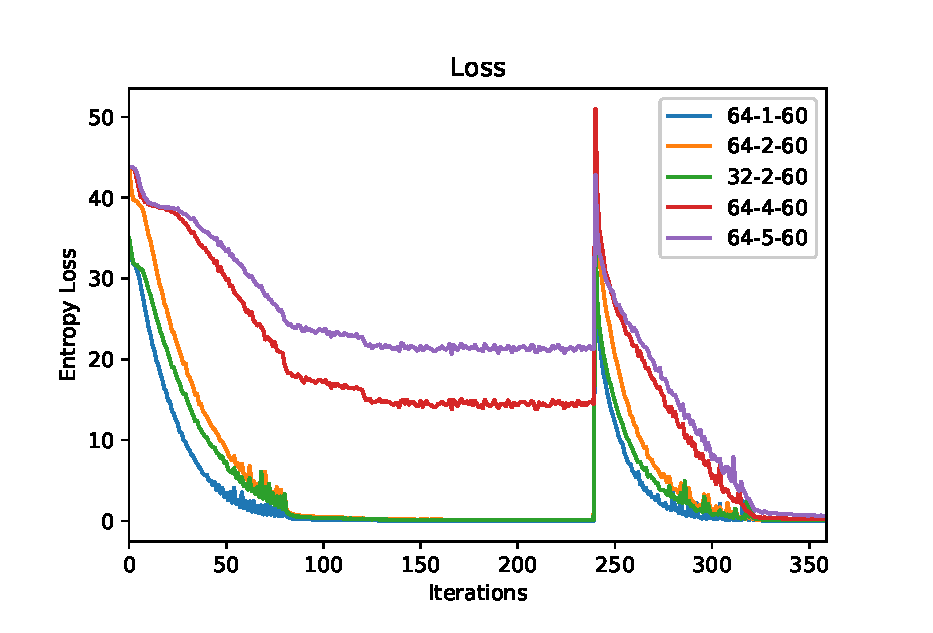
\includegraphics[width=1\textwidth]{figure/loss}
\caption{交叉熵误差随着迭代次数变化曲线}
\label{fig:loss}
\end{figure}
但是在绝对速度的比较上,训练过程所需的绝对时间还是与节点数成反比的,毕竟有更多的节点来分担
计算任务。例如单机训练需要花费22个小时,采用5个节点分布式训练只需要花费5个小时左右。

以上是采用单机训练和多机分布式训练的差异。对于最终训练结果,不管采用单机还是分布式,都会收敛到
一个相近的误差,即虽然过程有差异,但结果差异不大。证明了分布式训练是一种可行的加快训练速度的
方法。

\subsubsection{测试}
表\ref{tab:test}为在Market1501测试集上的测试结果:
\begin{table}[]
\centering
\caption{Market1501测试结果}
\label{tab:test}
\begin{tabular}{@{}lllll@{}}
\toprule
        & Rank1 & Rank5 & Rank10 & mAP  \\ \midrule
64-1-60 & 91.4  & 97.1  & 98.1   & 77.2 \\
64-2-60 & 89.6  & 96.3  & 97.8   & 75.2 \\
32-2-60 & 90.5  & 96.7  & 98.0   & 76.8 \\
64-4-60 & 89.5  & 96.1  & 96.7   & 75.4 \\
64-5-60 & 89.9  & 96.3  & 97.2   & 75.6 \\ \bottomrule
\end{tabular}
\end{table}

可以看出分布式训练结果的精度在误差允许的范围内。

\section{总结}
经过两个月紧张的毕业设计项目,作者在此过程中搭建了PyTorch分布式环境,完成了论文复现工作,在Market1501\cite{zheng2015scalable}数据库上进行实验。实现了 Q-Learning 强化学习算法,选择最优的摄像头部署方案。将深度行人重识别模型的训练算法改造成适用于多CPU集群的形式。

毕业设计的当前进度符合原计划的安排,在接下来的一段时间内应该继续完成剩余的实验项目,以及尽快完成毕业设计的论文写作和文献翻译工作。
%============= 参考文献 =====================
\include{body/reference}

\end{document}
%%%%%%%%%% 结束 %%%%%%%%%%
